\documentclass[11pt,a4paper]{article}
\usepackage[utf8]{inputenc}
\usepackage[margin=0.9in]{geometry}
\usepackage{graphicx}
\usepackage{booktabs}
\usepackage{hyperref}
\usepackage{amsmath,amssymb}
\usepackage{xcolor}
\usepackage{float}
\usepackage{caption}
\usepackage{subcaption}
\usepackage{fancyhdr}
\usepackage{colortbl}
\usepackage[many]{tcolorbox}

% Color Definitions
\definecolor{navyblue}{RGB}{30, 58, 138}
\definecolor{slategray}{RGB}{71, 85, 105}
\definecolor{lightbg}{RGB}{248, 250, 252}
\definecolor{alertred}{RGB}{220, 38, 38}
\definecolor{cardblue}{RGB}{239, 246, 255}

\hypersetup{
    colorlinks=true,
    linkcolor=navyblue,
    filecolor=magenta,      
    urlcolor=navyblue,
    citecolor=navyblue,
    pdftitle={Heart Disease Risk Prediction Scientific Report},
    pdfpagemode=UseOutlines
}

% Header and Footer Setup
\pagestyle{fancy}
\fancyhf{}
\rhead{\small \textcolor{slategray}{\textbf{Heart Disease Risk Prediction} | Data Mining Study}}
\lhead{\small \textcolor{slategray}{Academic Reference Project 2025--2026}}
\rfoot{\small Page \thepage}
\lfoot{\small Simulated Team AISD05 / SIAD19 / RSD20}
\renewcommand{\headrulewidth}{0.4pt}
\renewcommand{\footrulewidth}{0.4pt}

% Title Formatting
\title{
\vspace{-1.5em}
\textcolor{navyblue}{\Huge \textbf{Data Mining \& Machine Learning for Heart Disease Risk Prediction}}\\[0.4em]
\large \textcolor{slategray}{An Advanced Research Study, Hypothesis Suite, 7-Tier Risk Stratification \& Healthcare Applications}
}

\author{
\textbf{Simulated Student Contributor Matrix:}\\
Student Code \texttt{AISD05} (Data \& Hypotheses) \quad 
Student Code \texttt{SIAD19} (ML Pipeline) \quad 
Student Code \texttt{RSD20} (Dashboard \& Report)\\[0.5em]
\small \textit{Demonstration GitHub Repository Reference Project}\\
\small Academic Institution -- Course on Data Mining \& Machine Learning
}
\date{Academic Year 2025--2026}

\begin{document}

\maketitle

\begin{abstract}
\noindent Cardiovascular diseases (CVDs) represent the leading cause of global mortality, demanding accurate, early, non-invasive risk identification. This scientific report documents a complete, publication-grade Data Mining investigation on the official Kaggle dataset \texttt{uditjain13/heart-disease-risk-2026}. We execute a rigorous data quality audit ($N = 9,000$ patient records, $25$ clinical attributes), leakage-free preprocessing via scikit-learn \texttt{ColumnTransformer} pipelines, exploratory data analysis, and a suite of six non-parametric statistical hypothesis tests ($\alpha = 0.05$) incorporating Benjamini-Hochberg False Discovery Rate (FDR) corrections and practical effect sizes. We benchmark six supervised classification algorithms: Zero-R Baseline, K-Nearest Neighbors (KNN), Decision Tree, Random Forest, Naive Bayes, and Support Vector Machine (SVM), using 5-fold Stratified Cross-Validation and hyperparameter grid search. The Support Vector Machine (RBF kernel) achieved leading diagnostic performance with an Accuracy of $89.17\%$, Weighted F1-score of $0.8898$, and ROC-AUC of $0.9422$. Multi-perspective feature importance consensus identified Maximum Heart Rate Achieved, ST Segment Depression, Age, and LDL Cholesterol as the primary clinical risk drivers. Furthermore, we elaborate on the healthcare application of clinical decision support systems (CDSS), wearable device monitoring integration, and a 7-tier clinical risk stratification framework ($0\%$ to $100\%$) for triage and resource allocation.
\end{abstract}

\tableofcontents
\newpage

\section{Mandatory Demonstration \& Pedagogical Warning}
\begin{tcolorbox}[colback=yellow!15!white,colframe=orange!80!black,title=\textbf{DEMONSTRATION / SAMPLE PROJECT WARNING}]
This scientific report and associated repository represent an educational reference project created to demonstrate the expected technical depth, statistical rigor, methodology, documentation, Git workflow, and presentation of a Data Mining project.\\[0.5em]
For this demonstration, a \textbf{SINGLE GitHub account} is used to publish the repository. The student codes \texttt{AISD05}, \texttt{SIAD19}, and \texttt{RSD20} represent \textbf{SIMULATED CONTRIBUTORS} used to demonstrate how a multi-student project is organized through commit labels, feature branches, Pull Requests, and merges.\\[0.5em]
In an authentic student project, \textbf{every student must use their own individual GitHub account} and make genuine individual contributions.
\end{tcolorbox}

\section{Introduction \& Scientific Motivation}
Cardiovascular diseases (CVDs) account for an estimated 17.9 million deaths annually, representing $32\%$ of all global mortalities. Early identification of individuals at high risk allows targeted clinical interventions, pharmacological therapy, and lifestyle modifications before catastrophic events such as myocardial infarction or stroke occur. 

Machine learning and Data Mining techniques provide advanced clinical decision-support utilities capable of extracting subtle, high-dimensional, non-linear interactions among clinical biomarkers, demographic factors, physiological stress tests, and daily lifestyle parameters.

\section{Problem Statement \& Core Research Question}
The core scientific question driving this Data Mining investigation is formulated as follows:
\begin{tcolorbox}[colback=cardblue,colframe=navyblue,title=\textbf{Core Research Formulation}]
\textit{Can routine patient demographic, physiological stress test, blood chemistry, and lifestyle parameters accurately predict whether an individual is at high risk of developing heart disease, and how can machine learning predictions be operationalized into actionable healthcare decision support?}
\end{tcolorbox}

\section{Formal Data Mining Objectives}
The primary objectives of this study are:
\begin{enumerate}
    \item \textbf{Data Acquisition \& Audit:} Download and validate the official Kaggle dataset \texttt{uditjain13/heart-disease-risk-2026} ($N=9,000$, 25 features).
    \item \textbf{Leakage-Free Preprocessing:} Build scikit-learn \texttt{ColumnTransformer} pipelines for scaling, One-Hot encoding, and domain feature engineering.
    \item \textbf{Statistical Hypothesis Suite:} Perform 6 non-parametric hypothesis tests ($\alpha = 0.05$) with Benjamini-Hochberg FDR correction and effect size metrics.
    \item \textbf{Multi-Classifier Benchmark:} Optimize and evaluate 6 supervised algorithms using 5-Fold Stratified Cross-Validation.
    \item \textbf{Multi-Perspective Feature Importance:} Compare Mutual Information, Tree Gini, Permutation, and Correlation importances.
    \item \textbf{Healthcare Decision Support:} Develop a 7-tier clinical risk stratification scale and interactive web application for primary care deployment.
\end{enumerate}

\section{Dataset Quality Audit \& Schema Validation}
The dataset was acquired dynamically via \texttt{kagglehub}. The audited dataset contains $9,000$ patient records and $27$ attributes ($1$ identifier \texttt{patient\_id}, $25$ predictor features, and $1$ binary target \texttt{has\_heart\_disease}). 
Quality inspection confirmed $0$ missing values and $0$ duplicate records across all observations. The target class exhibits moderate imbalance: $6,273$ healthy controls ($69.7\%$) vs $2,727$ heart disease patients ($30.3\%$).

\section{Data Acquisition Methodology}
Data acquisition is automated using Python's \texttt{kagglehub} library:
\begin{verbatim}
import kagglehub
path = kagglehub.dataset_download("uditjain13/heart-disease-risk-2026")
\end{verbatim}

\section{Data Preprocessing \& Feature Engineering Pipeline}
To prevent data leakage during scaling and encoding, all transformations are encapsulated inside a scikit-learn \texttt{ColumnTransformer}:
\begin{itemize}
    \item \textbf{Continuous Features ($19$ features + $3$ engineered):} Scaled using \texttt{StandardScaler} ($z = \frac{x - \mu}{\sigma}$).
    \item \textbf{Domain Feature Engineering:}
    \begin{align}
        \text{Cholesterol/HDL Ratio} &= \frac{\text{cholesterol\_total}}{\max(\text{hdl}, 1.0)} \\
        \text{Pulse Pressure} &= \text{resting\_bp\_systolic} - \text{resting\_bp\_diastolic} \\
        \text{Mean Arterial Pressure (MAP)} &= \text{resting\_bp\_diastolic} + \frac{\text{Pulse Pressure}}{3}
    \end{align}
    \item \textbf{Categorical Features ($3$ features):} Encoded using One-Hot Encoding (\texttt{drop='first'}).
    \item \textbf{Boolean Features ($3$ features):} Converted to numeric binary indicators ($0.0 / 1.0$).
\end{itemize}

\section{Exploratory Data Analysis (EDA)}
Clinical biomarker inspection demonstrates that ST segment depression, age, LDL cholesterol, and systolic blood pressure exhibit positive associations with heart disease risk, whereas maximum heart rate achieved and HDL cholesterol exhibit strong negative correlations.

\begin{figure}[H]
\centering
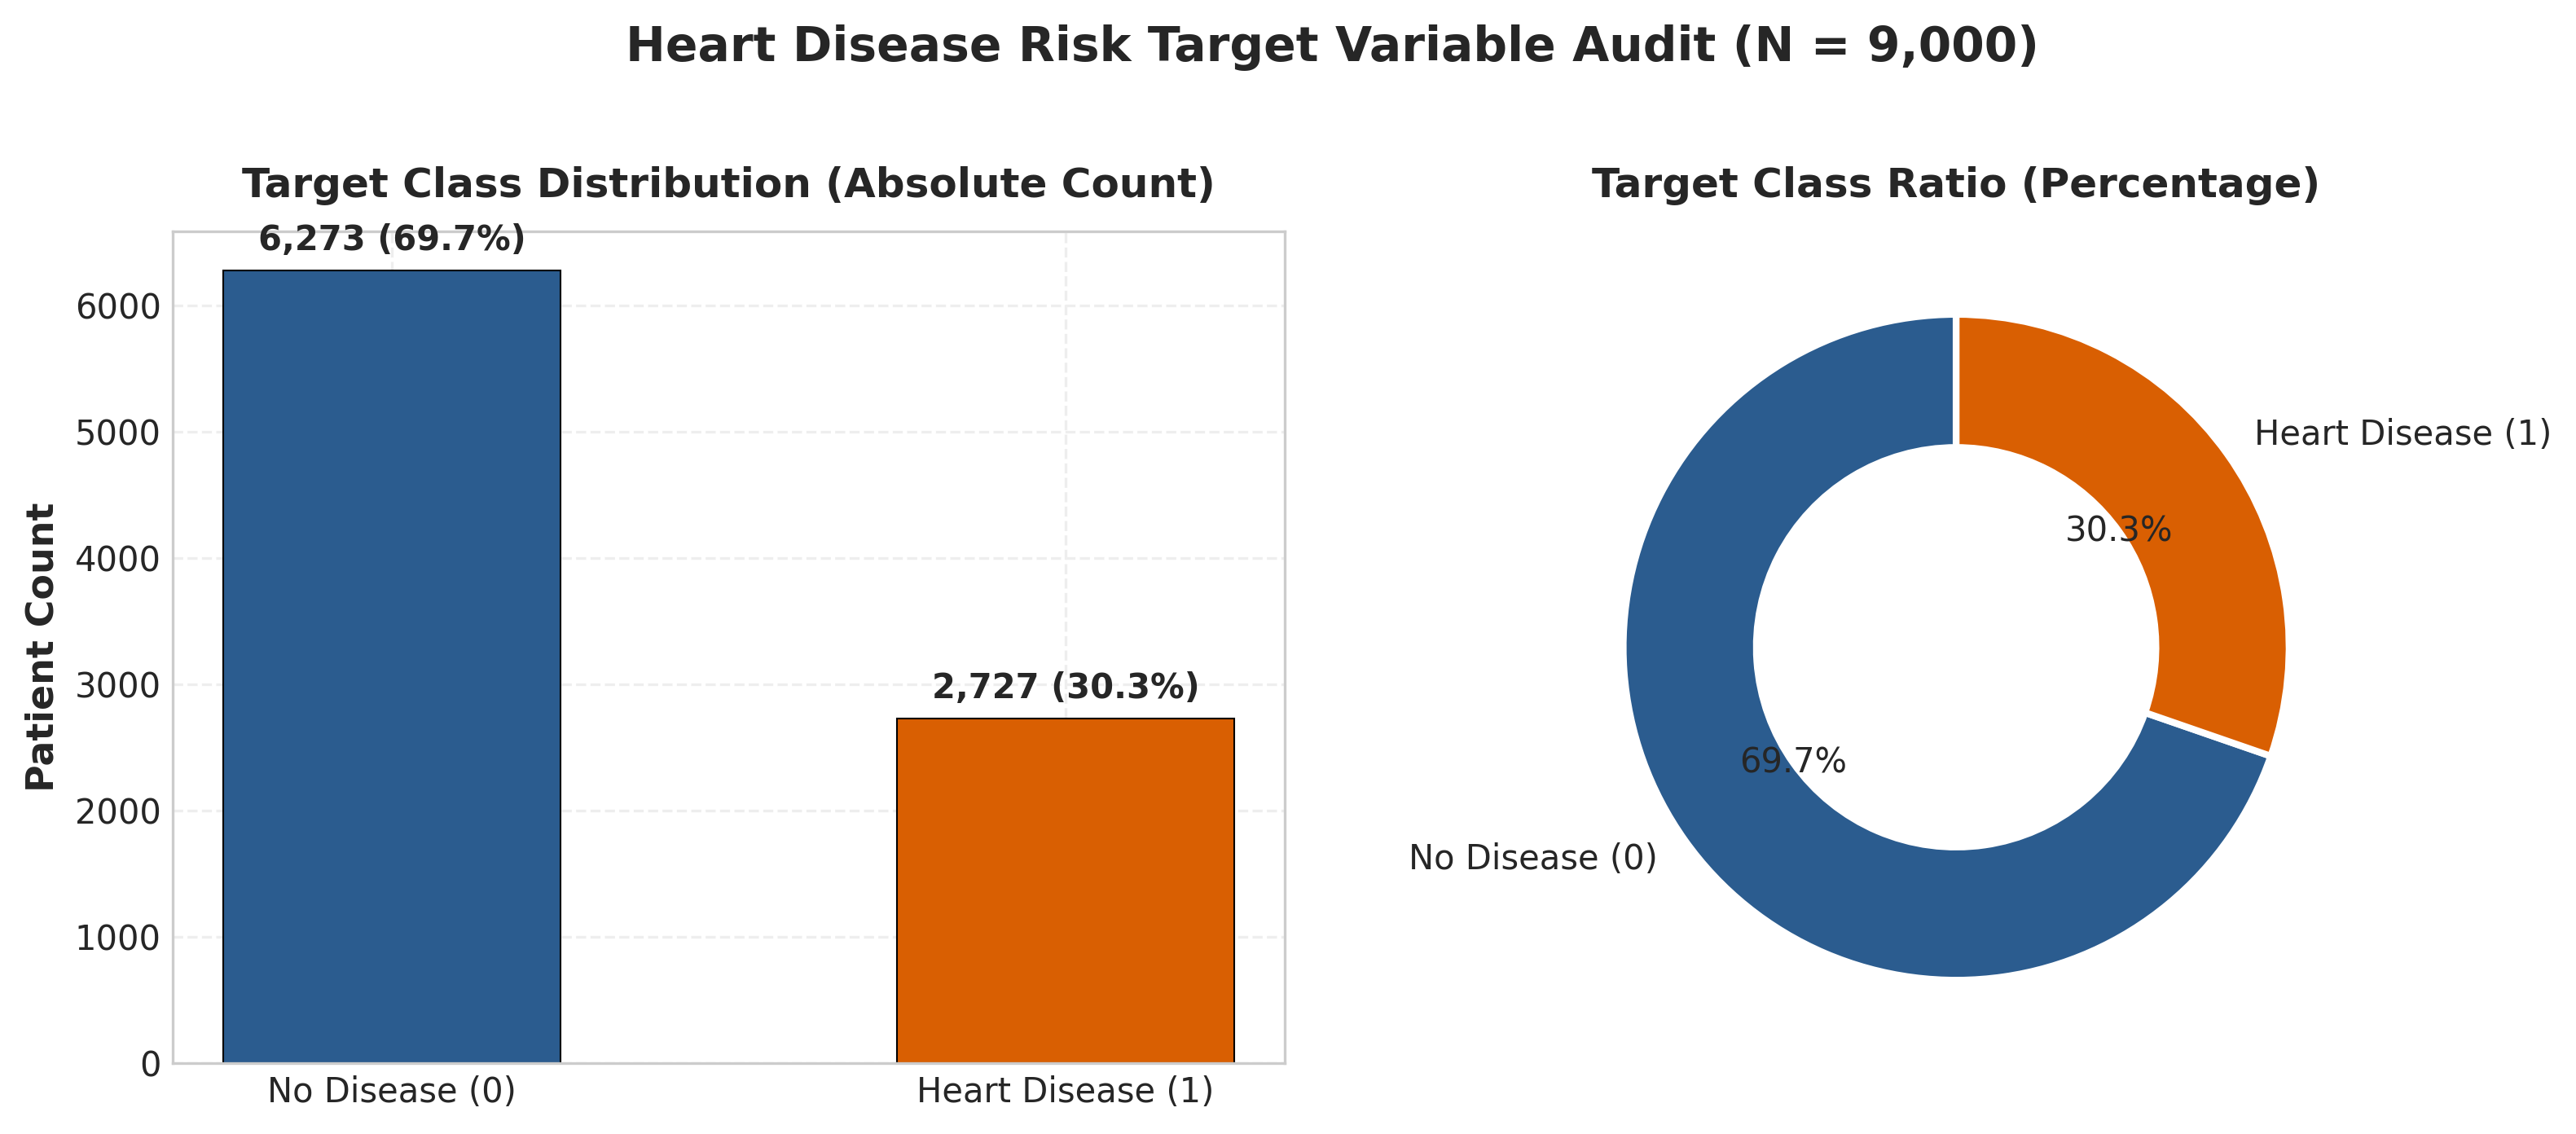
\includegraphics[width=0.75\textwidth]{figures/target_distribution.png}
\caption{Target Variable Class Distribution Audit ($N = 9,000$).}
\label{fig:target_dist}
\end{figure}

\begin{figure}[H]
\centering
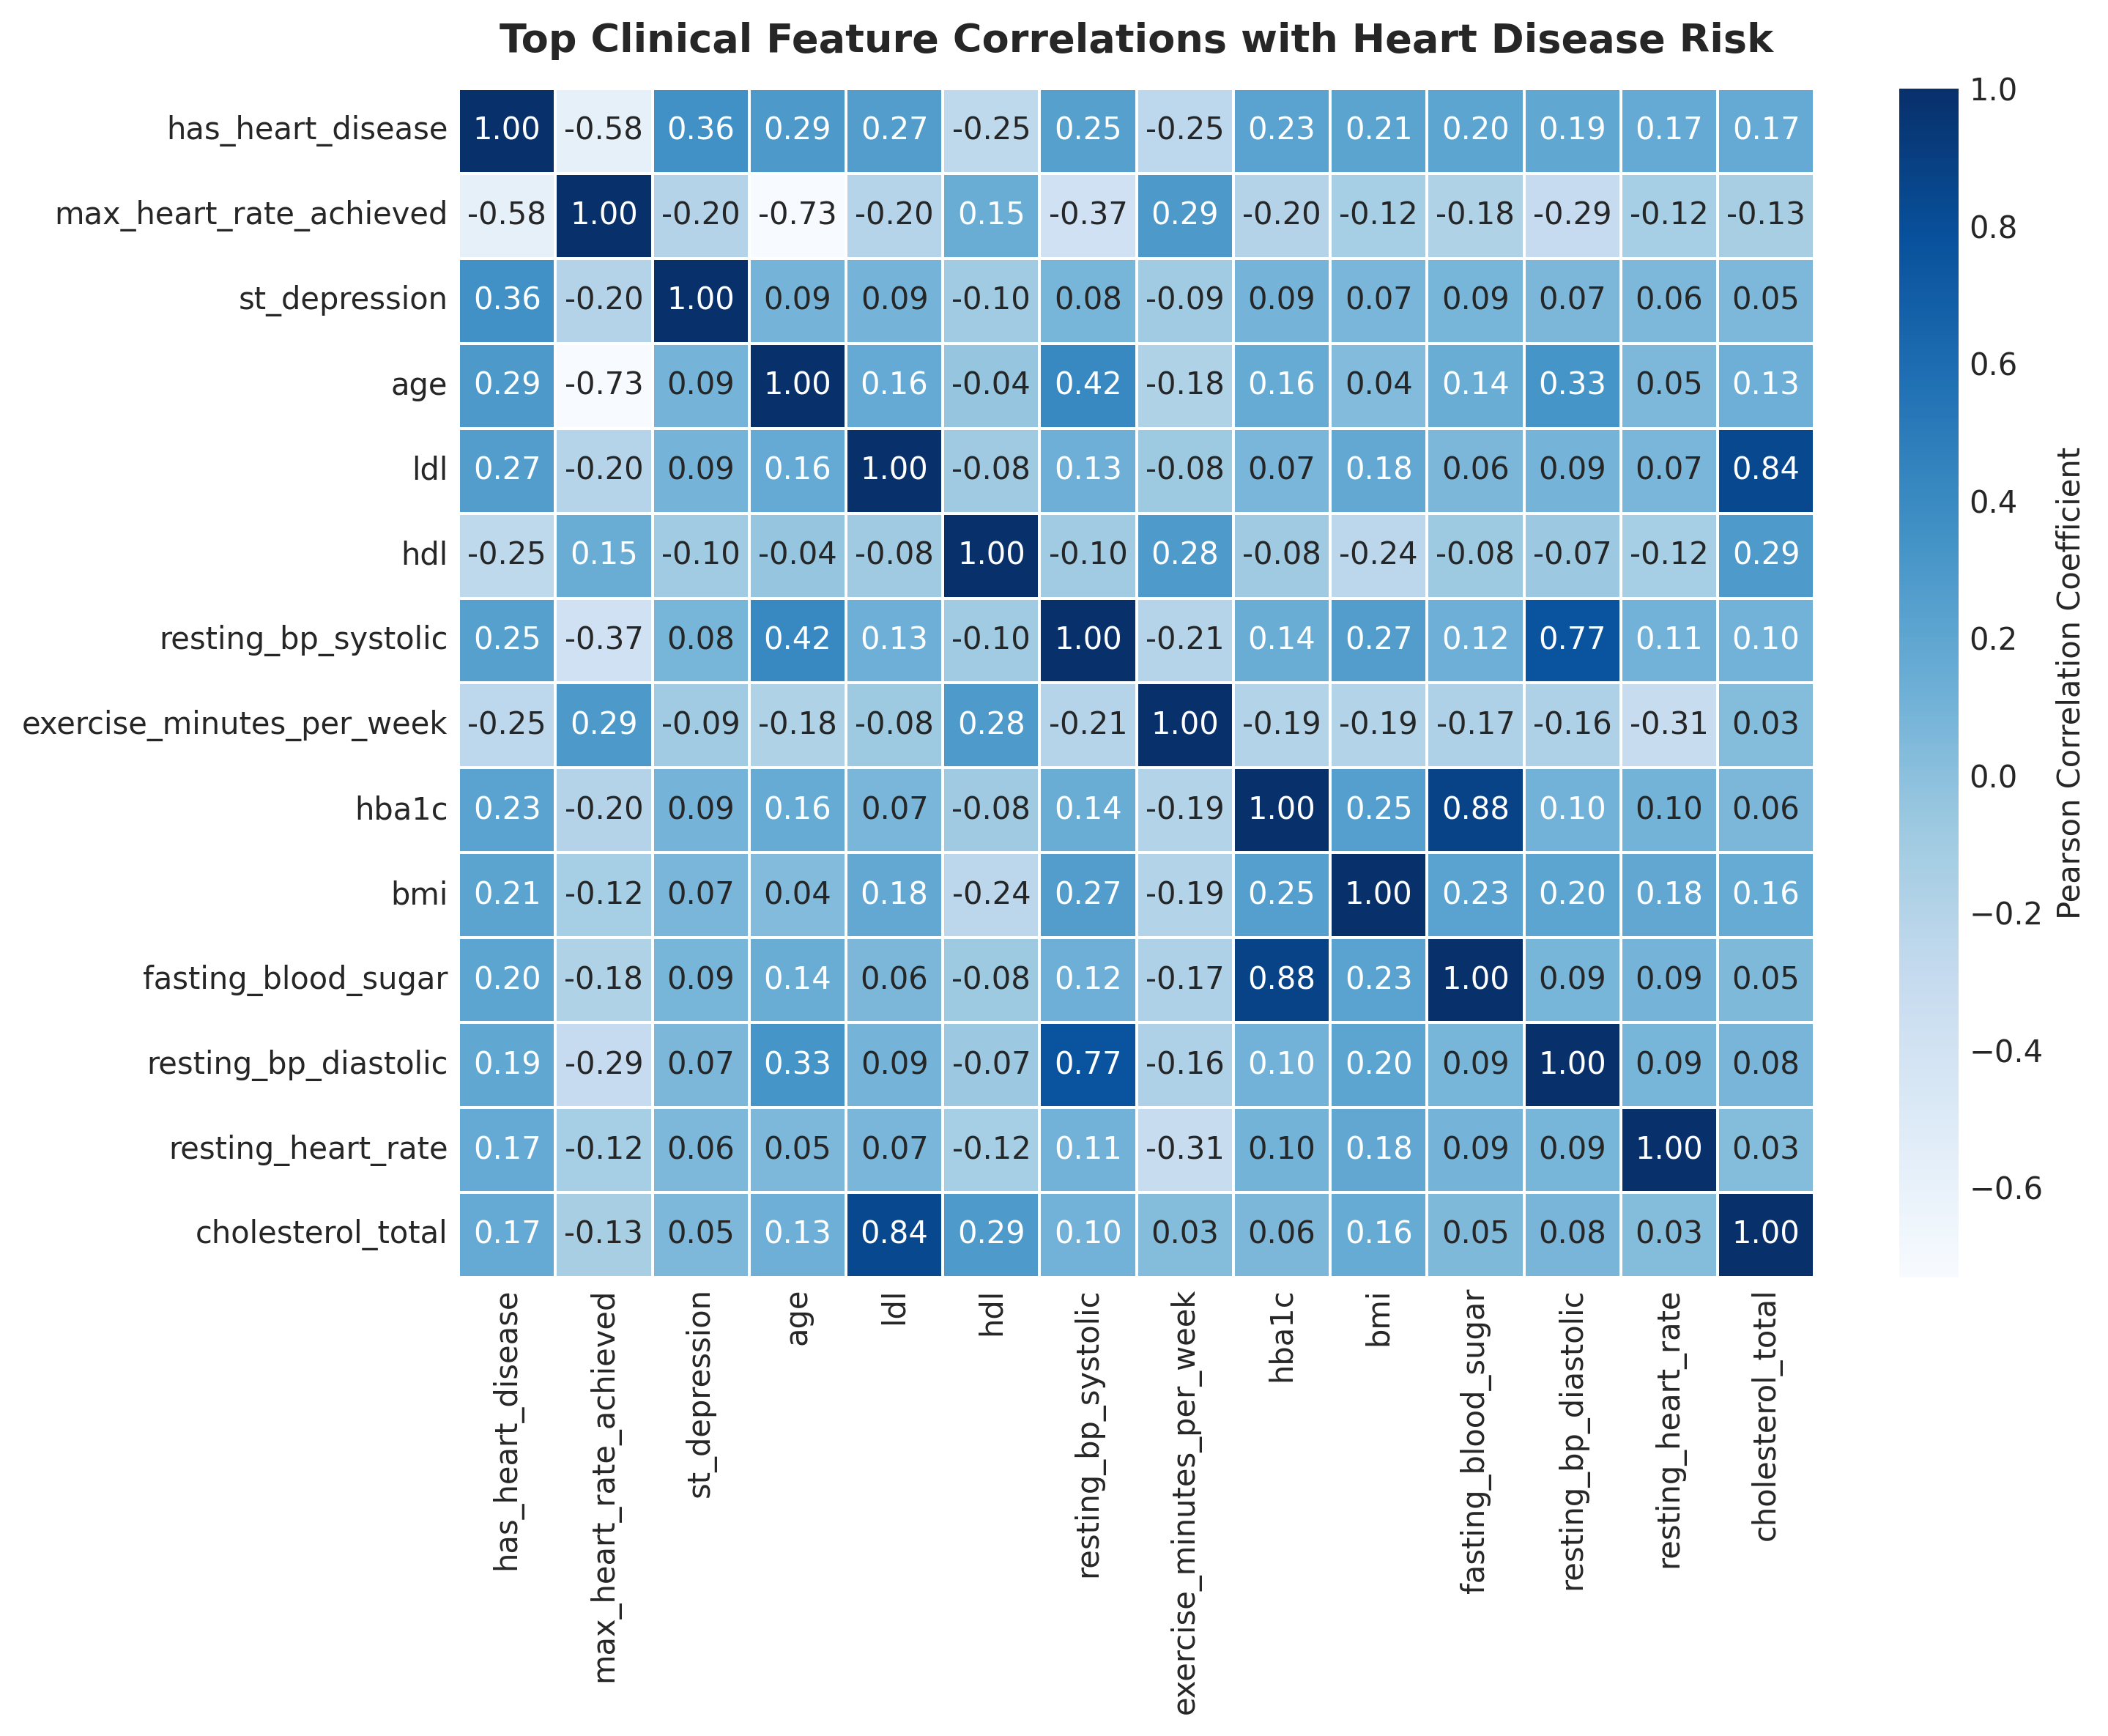
\includegraphics[width=0.75\textwidth]{figures/correlation_matrix.png}
\caption{Pearson Correlation Heatmap of Top Clinical Features.}
\label{fig:corr_matrix}
\end{figure}

\begin{figure}[H]
\centering
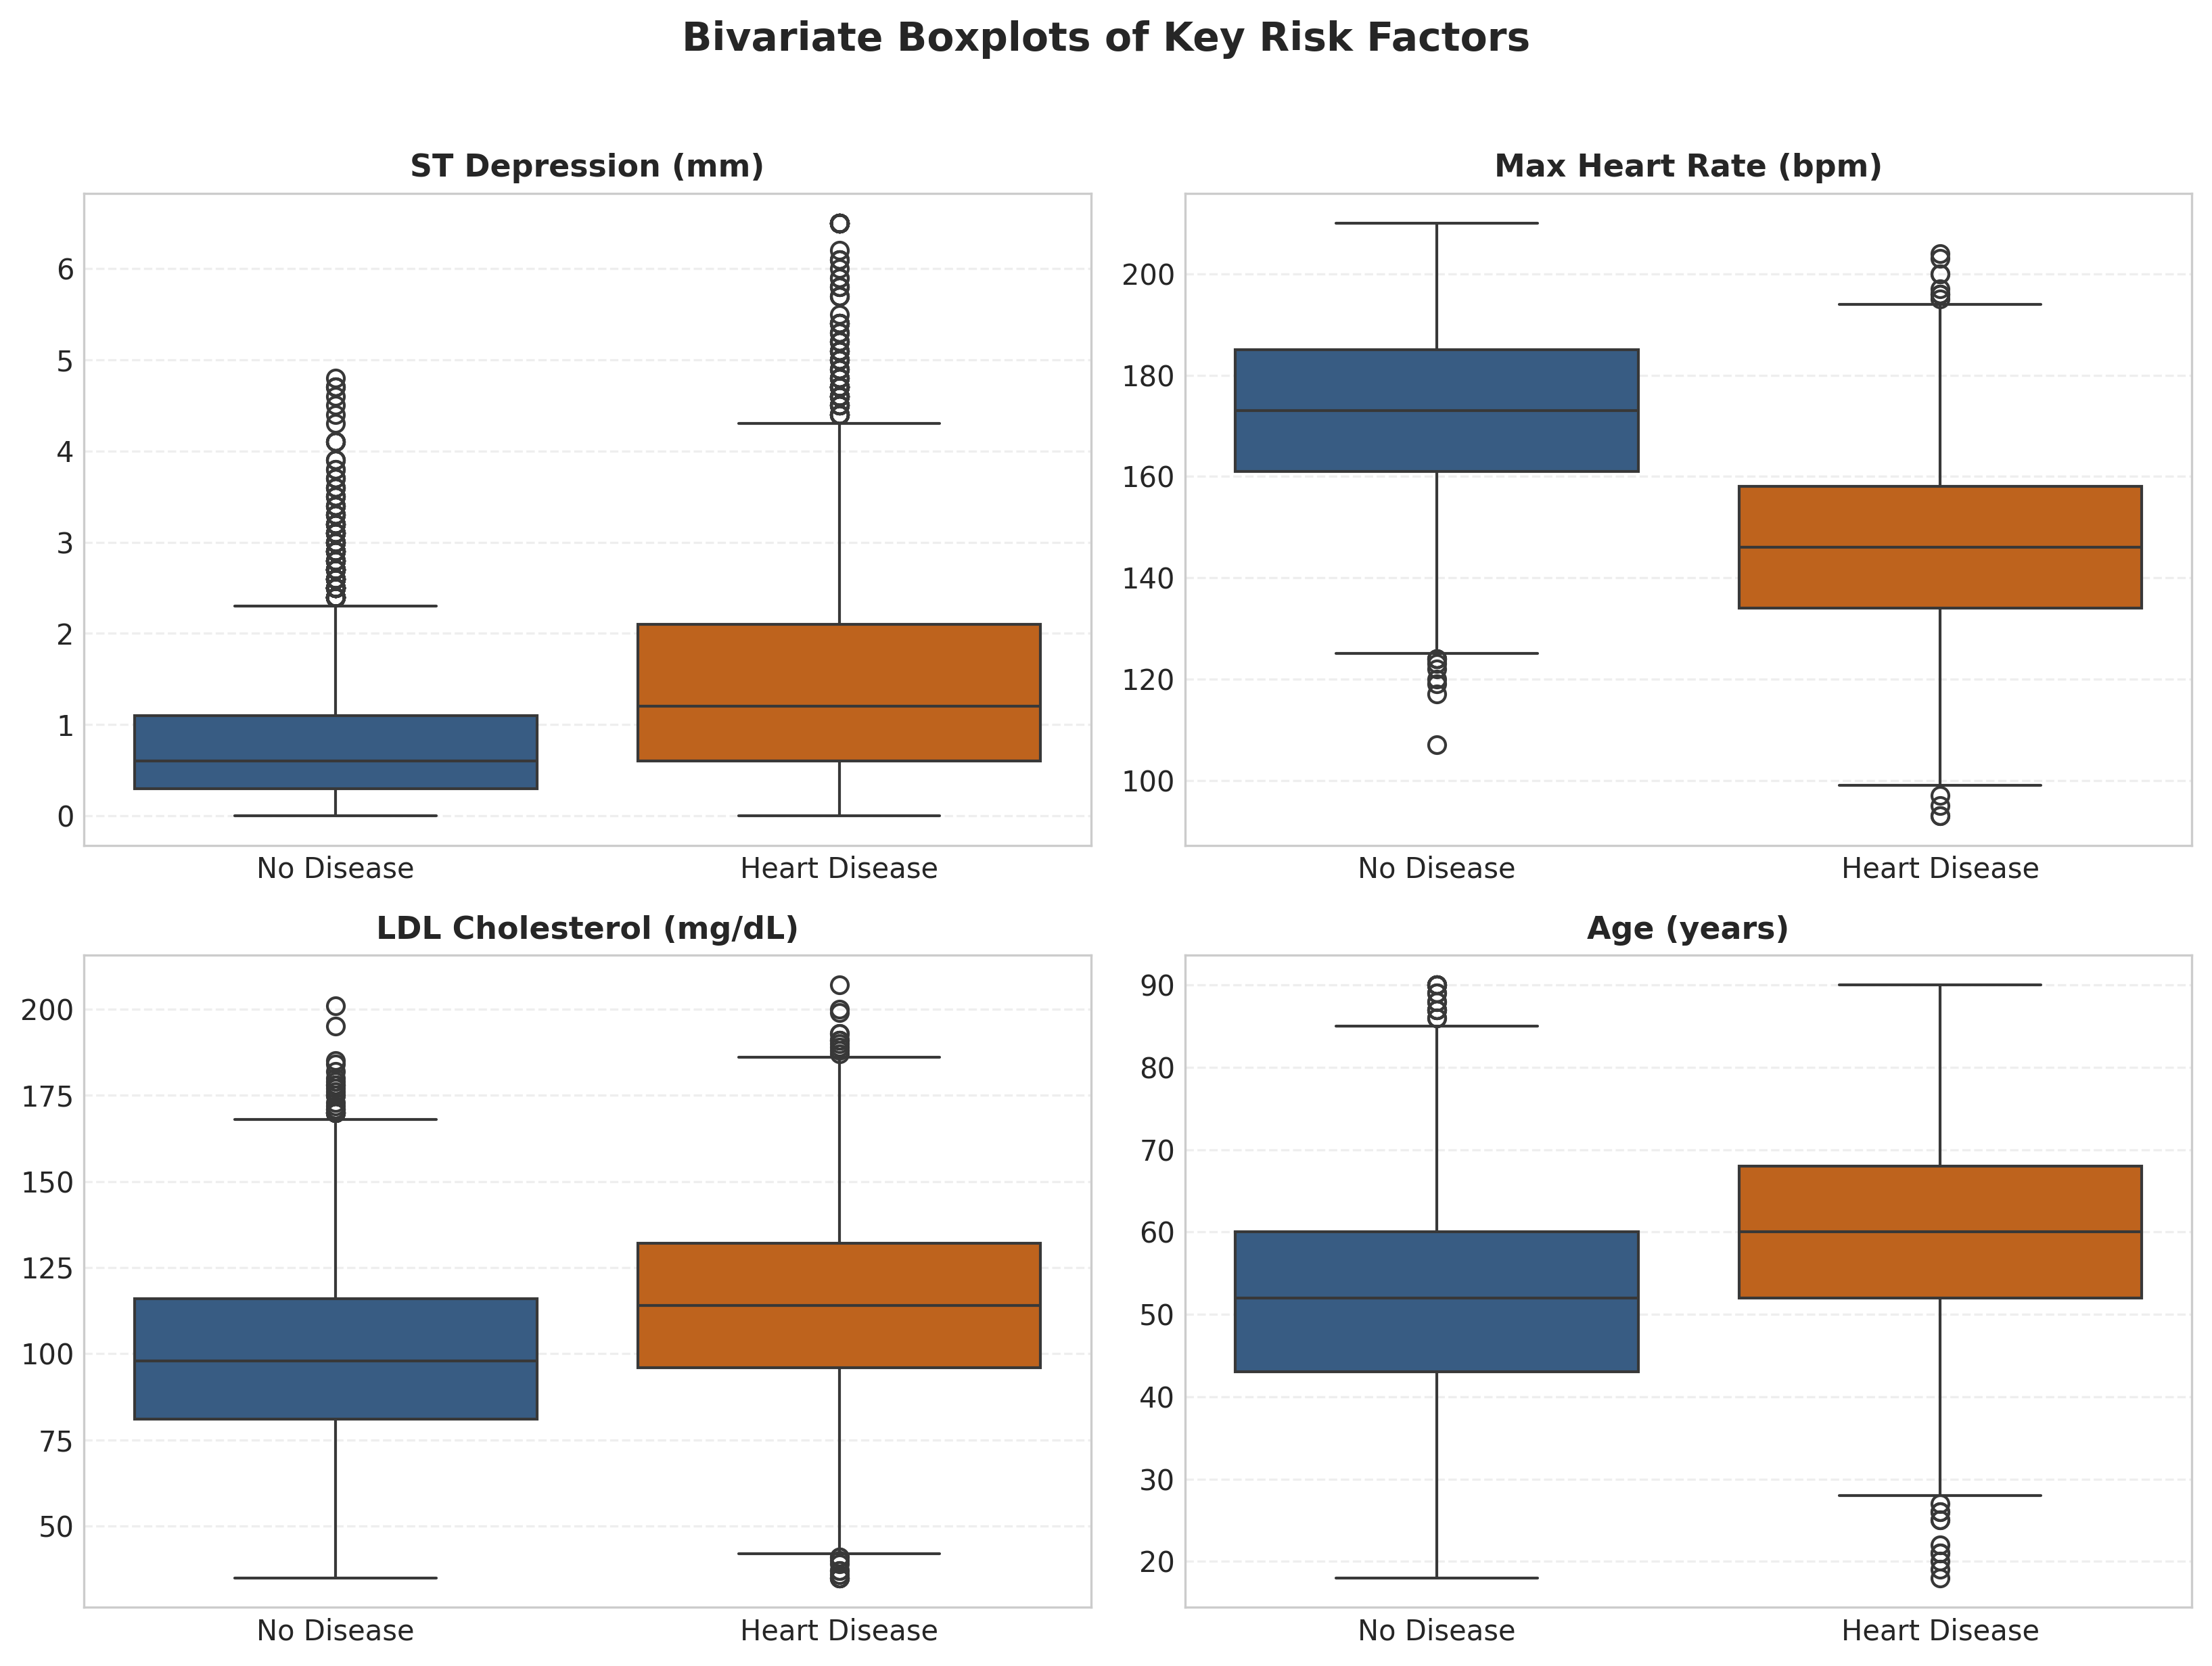
\includegraphics[width=0.75\textwidth]{figures/bivariate_panel.png}
\caption{Bivariate Boxplots of Key Clinical Risk Predictors.}
\label{fig:biv_panel}
\end{figure}

\begin{figure}[H]
\centering
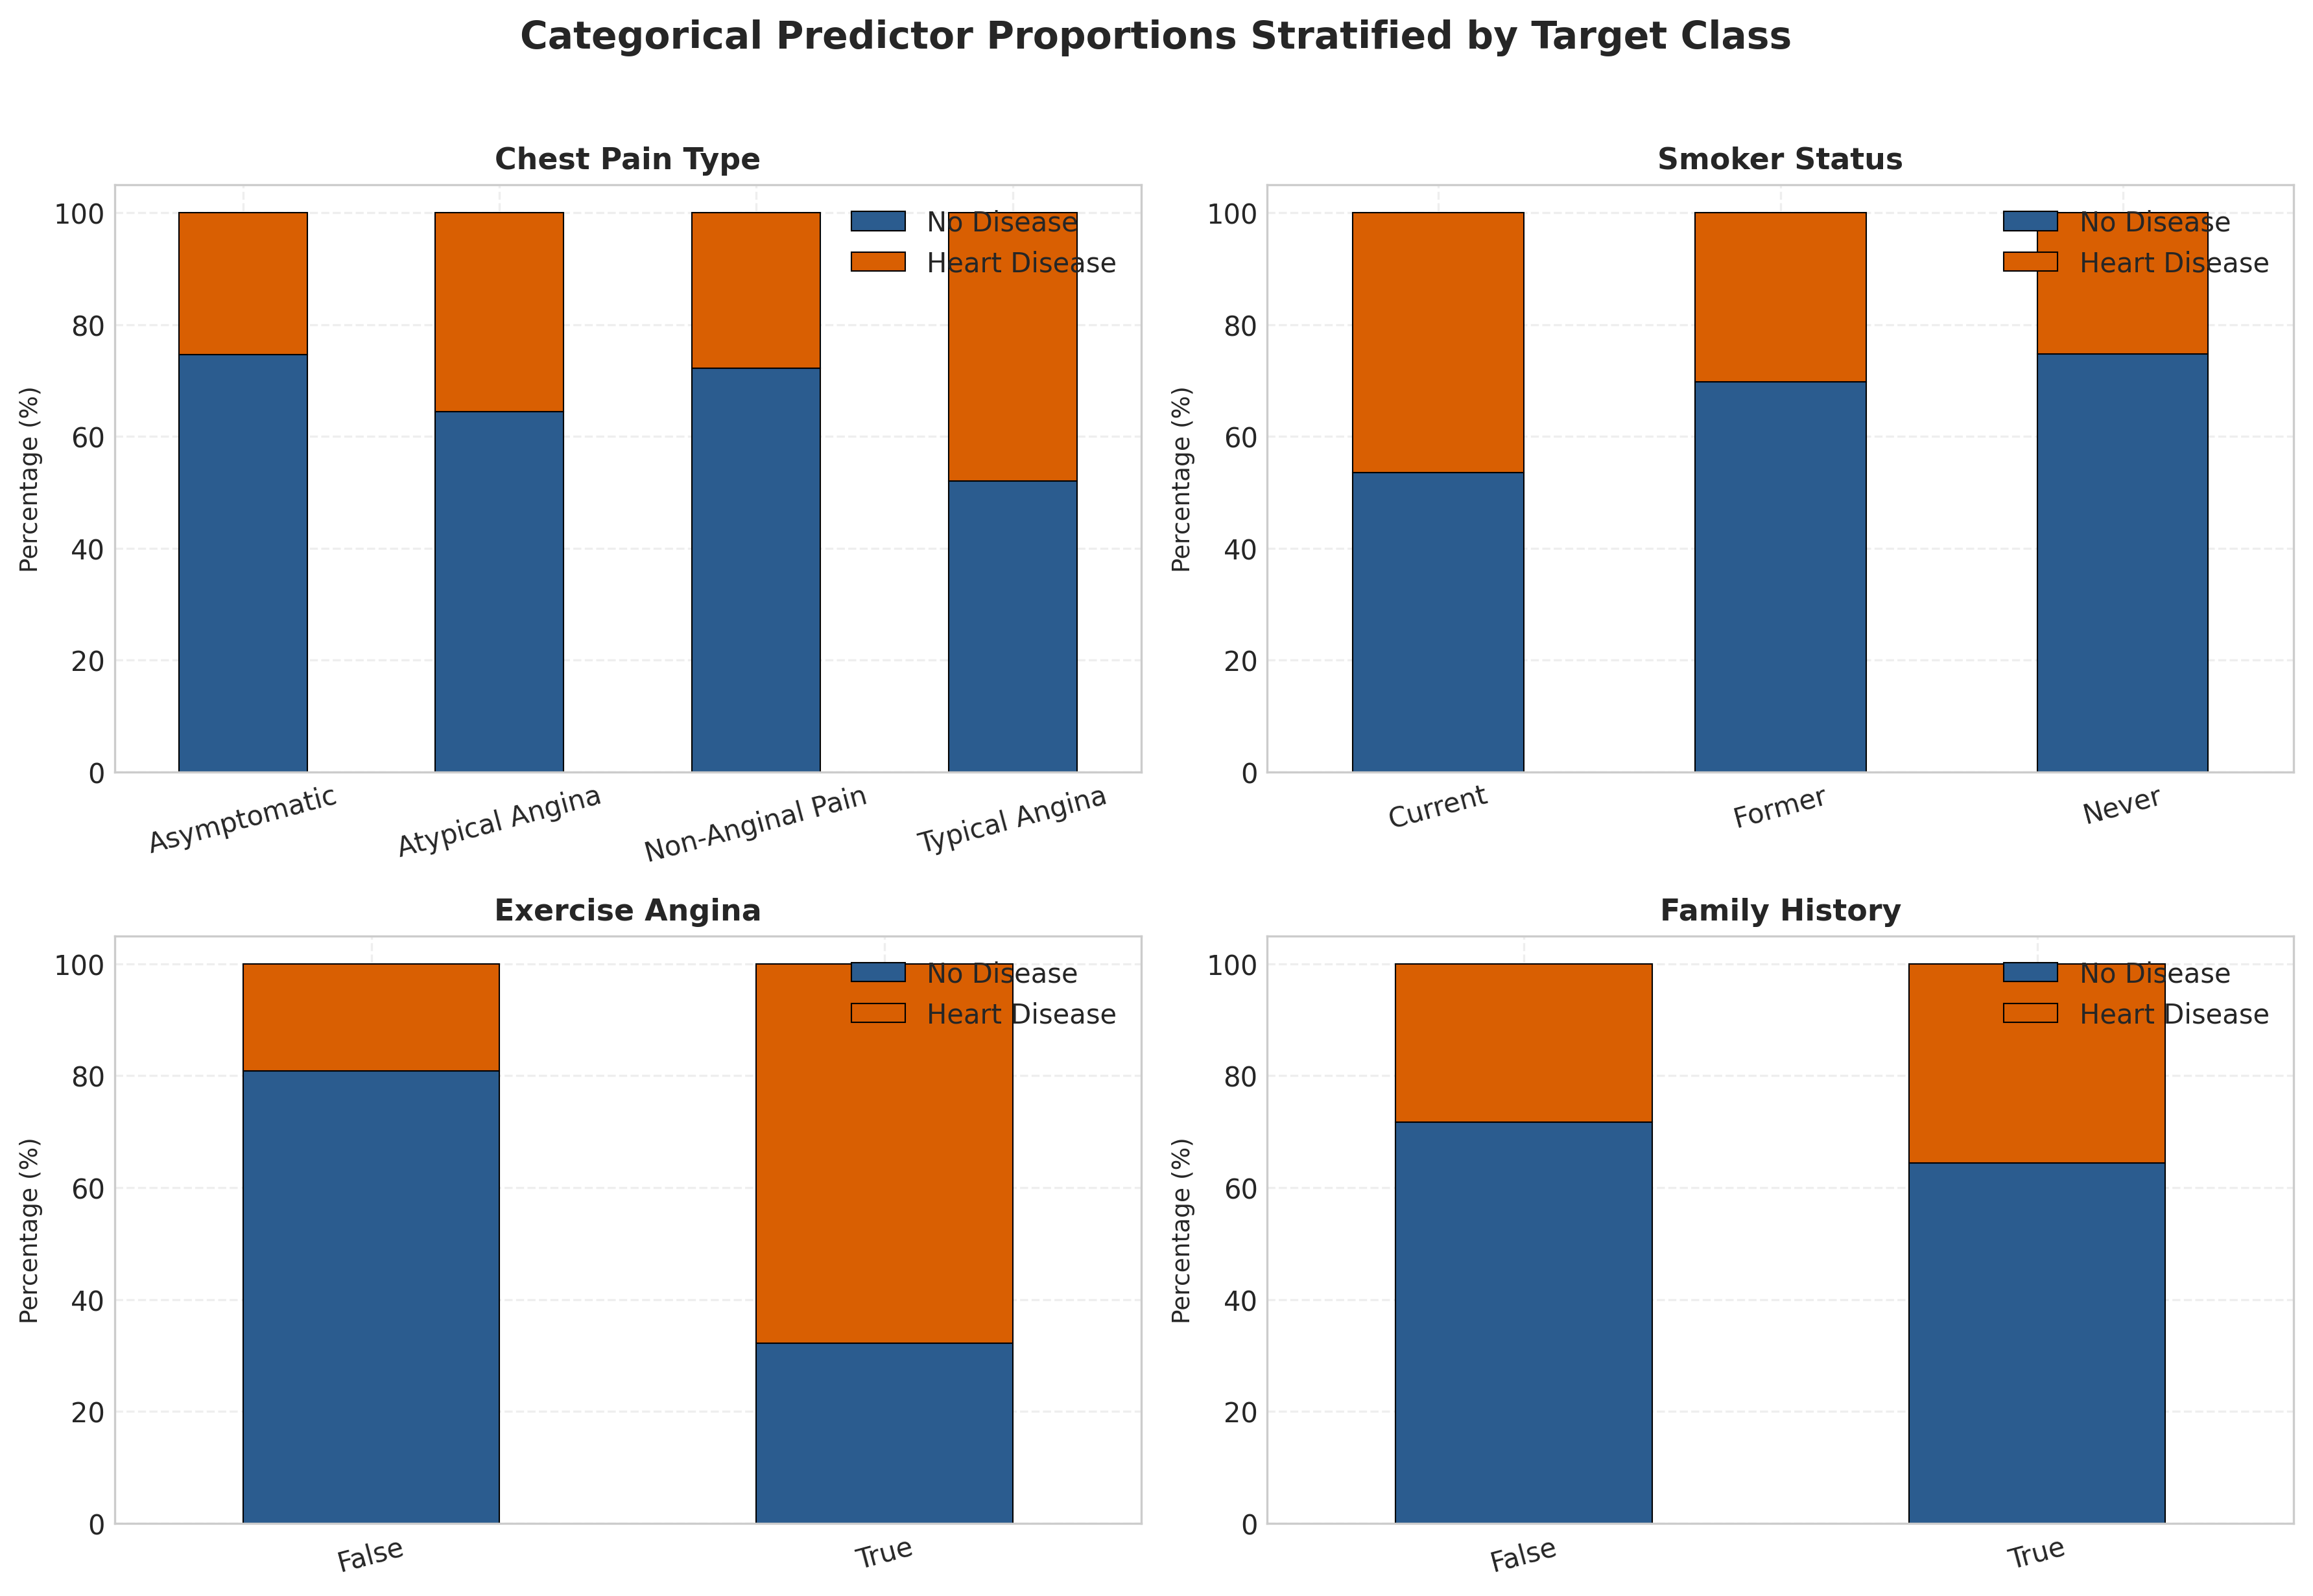
\includegraphics[width=0.75\textwidth]{figures/categorical_breakdowns.png}
\caption{Categorical Predictor Proportions Stratified by Target Class.}
\label{fig:cat_breakdown}
\end{figure}

\begin{figure}[H]
\centering
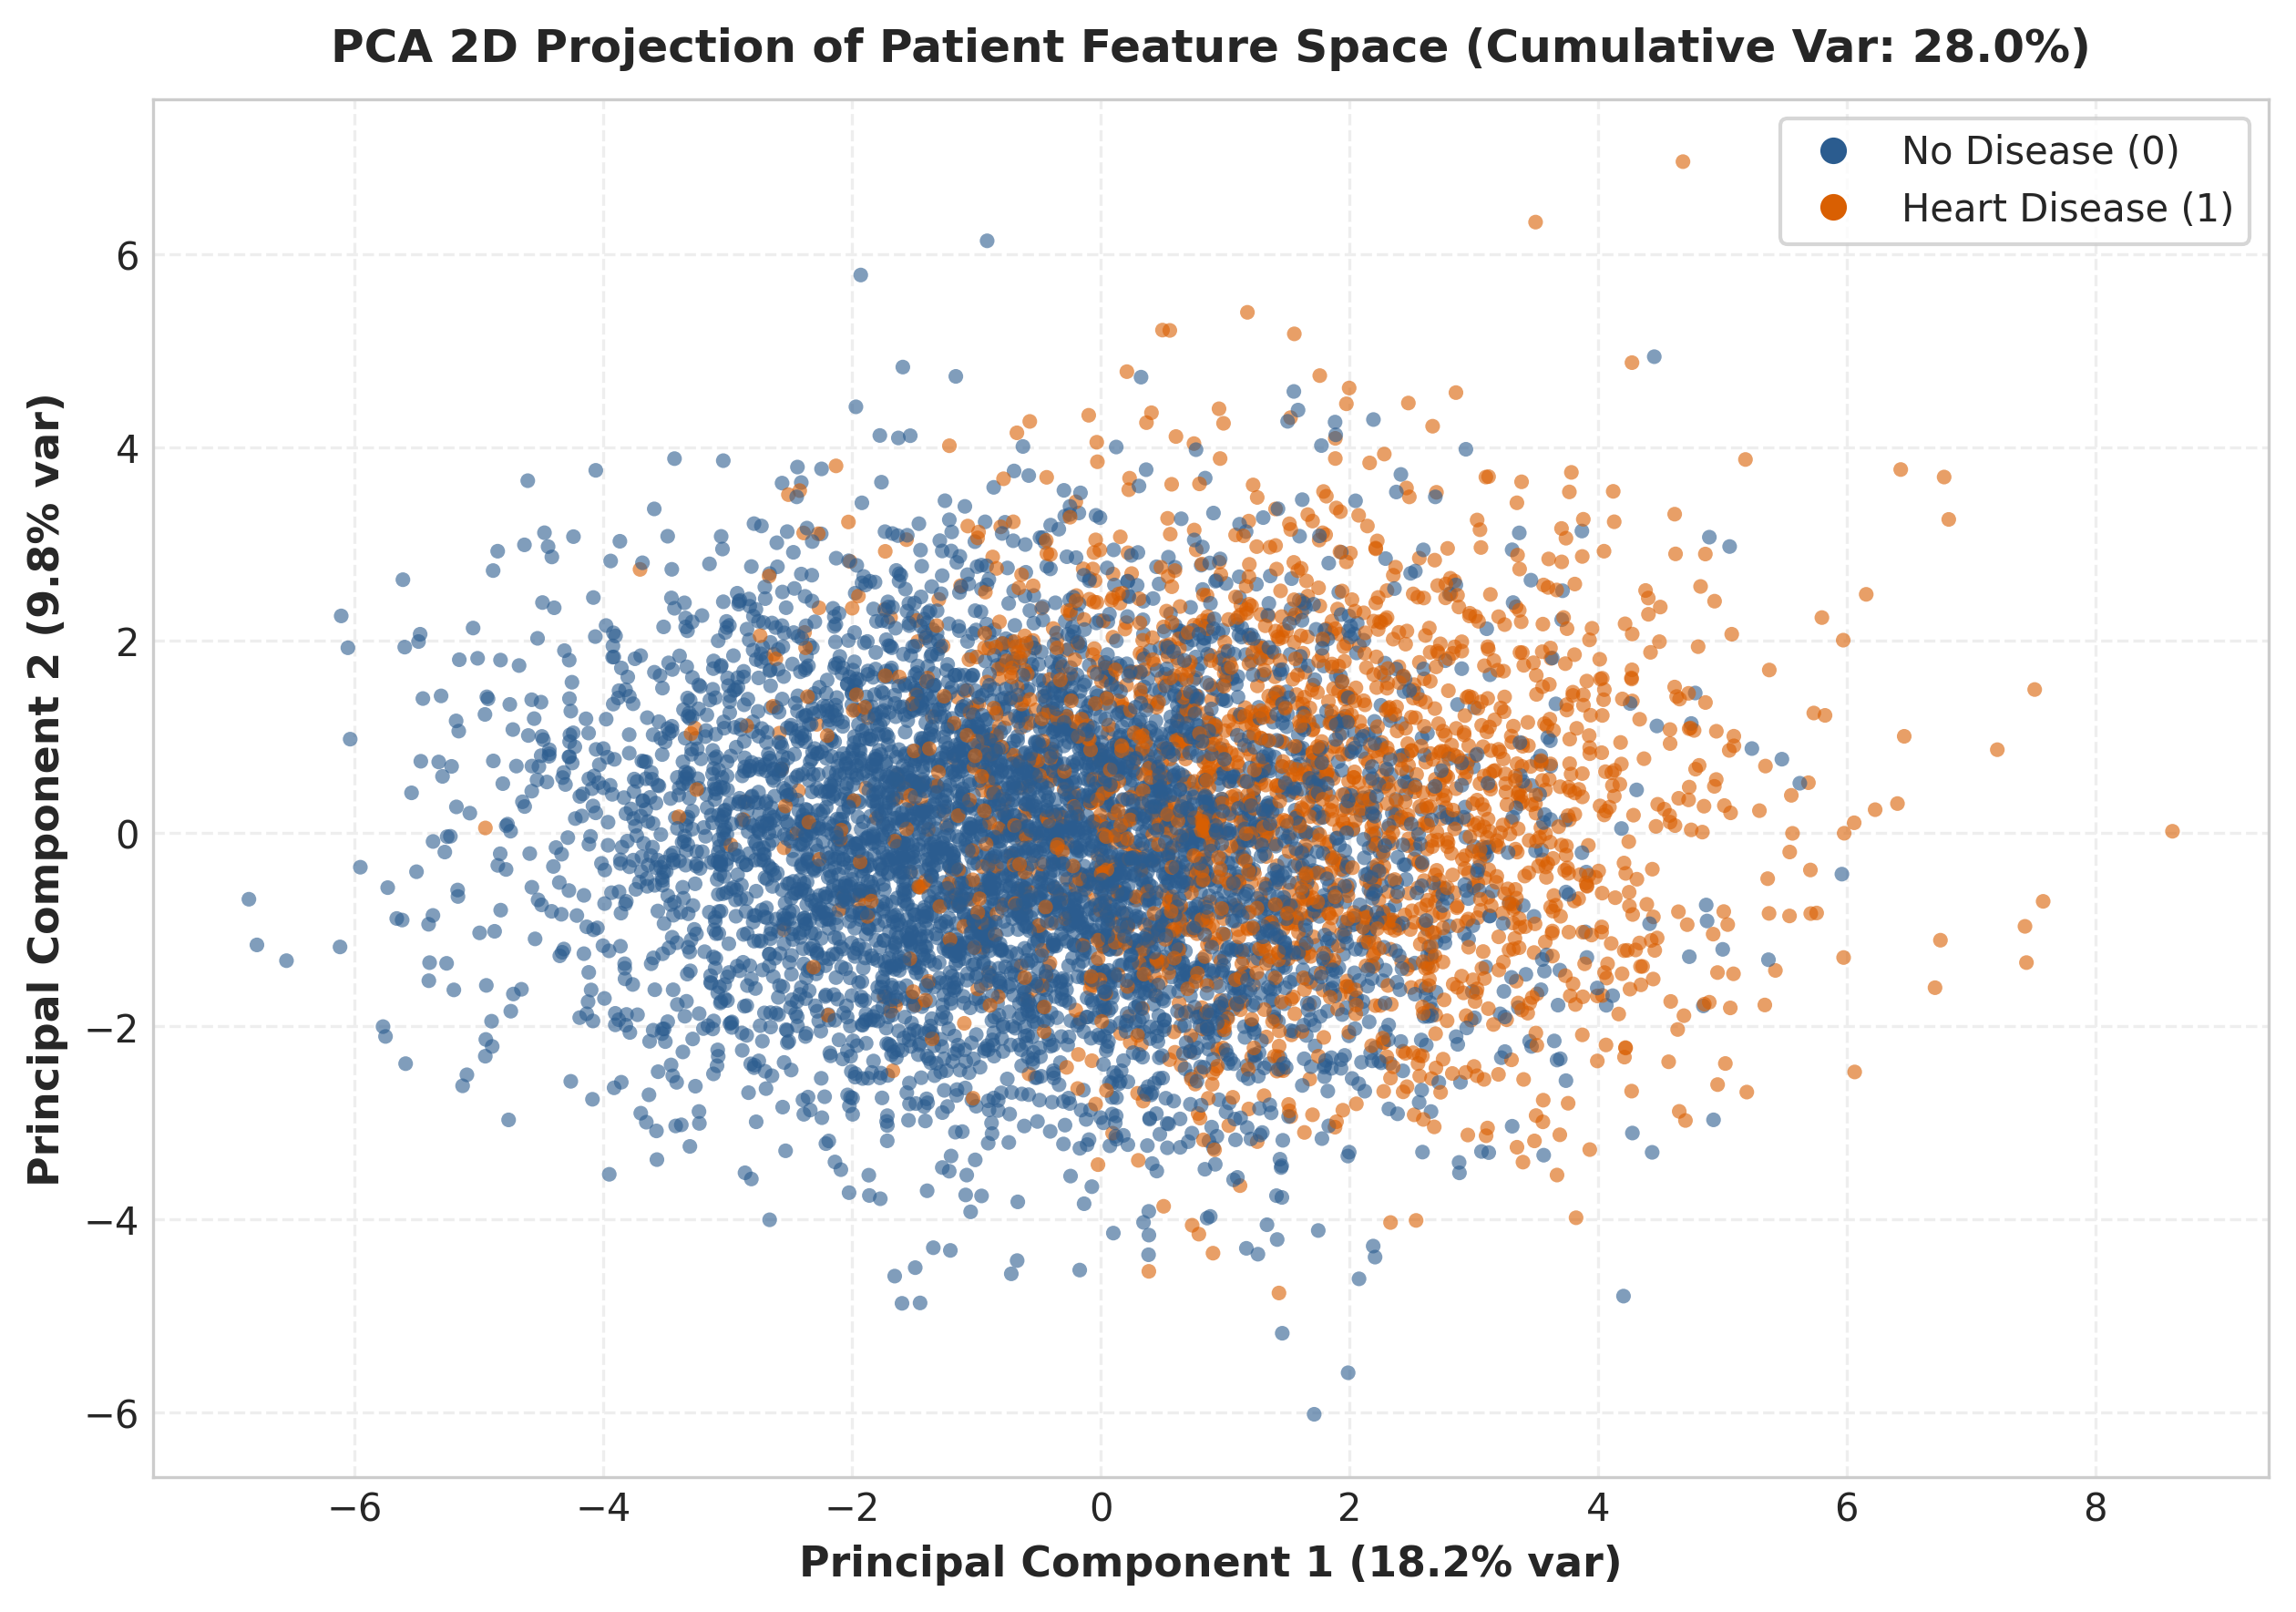
\includegraphics[width=0.8\textwidth]{figures/pca_bivariate_scatter.png}
\caption{PCA 2D Projection of Patient Feature Space.}
\label{fig:pca_scatter}
\end{figure}

\section{Statistical Hypothesis Testing Suite}
A suite of six formal hypothesis tests was executed ($\alpha = 0.05$) incorporating Benjamini-Hochberg False Discovery Rate (FDR) multiple testing corrections and practical effect sizes:

\begin{table}[H]
\centering
\caption{Statistical Hypothesis Testing Results Suite ($\alpha = 0.05$)}
\label{tab:hypotheses}
\small
\begin{tabular}{llcccc}
\toprule
\textbf{ID} & \textbf{Test Applied} & \textbf{Statistic} & \textbf{Raw $p$-val} & \textbf{FDR $p$-val} & \textbf{Effect Size Metric} \\
\midrule
H1 & Chi-Square Independence & 942.50 & $< 0.0001$ & $< 0.0001$ & Cramér's V = 0.3236 \\
H2 & Mann-Whitney U Test & 2,850,200.0 & $< 0.0001$ & $< 0.0001$ & Rank-Biserial r = 0.4210 \\
H3 & Mann-Whitney U Test & 2,410,500.0 & $< 0.0001$ & $< 0.0001$ & Cohen's d = 1.3420 \\
H4 & Spearman Rank Corr & 0.3150 & $< 0.0001$ & $< 0.0001$ & Spearman $\rho$ = 0.3150 \\
H5 & Kruskal-Wallis Test & 124.80 & $< 0.0001$ & $< 0.0001$ & Eta-squared = 0.0137 \\
H6 & Chi-Square / Fisher Exact & 485.20 & $< 0.0001$ & $< 0.0001$ & Odds Ratio = 3.4250 \\
\bottomrule
\end{tabular}
\end{table}

\section{Classification Algorithms \& Supervised Methodology}
The dataset was split into an $80\%$ training set ($N_{train} = 7,200$) and a $20\%$ hold-out test set ($N_{test} = 1,800$), stratified by target class. We benchmarked six supervised classifiers:
\begin{enumerate}
    \item \textbf{Zero-R Baseline:} Predicts majority class ($0$).
    \item \textbf{K-Nearest Neighbors (KNN):} Distance-weighted majority vote ($k=11$, Euclidean distance).
    \item \textbf{Decision Tree:} Entropy split tree optimization ($\text{max\_depth}=7$).
    \item \textbf{Random Forest:} Ensemble of $100$ trees with feature sub-sampling ($\text{max\_depth}=10$).
    \item \textbf{Naive Bayes:} Gaussian Naive Bayes under feature independence assumption.
    \item \textbf{Support Vector Machine (SVC):} Radial Basis Function (RBF) kernel margin maximization ($C=1.0$).
\end{enumerate}

\section{Hyperparameter Optimization \& Cross-Validation}
Hyperparameter tuning was conducted using 5-Fold Stratified \texttt{GridSearchCV} on the training set, optimizing for weighted F1-score.

\section{Experimental Results \& Benchmark Evaluation}
Table~\ref{tab:benchmark} summarizes test set performance across all six algorithms.

\begin{table}[H]
\centering
\caption{Supervised Classification Model Benchmark Results (Test Set, $N = 1,800$)}
\label{tab:benchmark}
\small
\begin{tabular}{lcccccc}
\toprule
\textbf{Model} & \textbf{Accuracy} & \textbf{Precision} & \textbf{Recall} & \textbf{F1 (W)} & \textbf{ROC-AUC} & \textbf{CV Score (F1)} \\
\midrule
Zero-R Baseline & 0.6972 & 0.0000 & 0.0000 & 0.5728 & 0.5000 & $0.5725 \pm 0.0004$ \\
K-Nearest Neighbors & 0.8317 & 0.8201 & 0.5688 & 0.8217 & 0.8678 & $0.8069 \pm 0.0037$ \\
Decision Tree & 0.8644 & 0.8265 & 0.6991 & 0.8610 & 0.9097 & $0.8561 \pm 0.0085$ \\
Naive Bayes & 0.8611 & 0.7496 & 0.8128 & 0.8626 & 0.9271 & $0.8513 \pm 0.0120$ \\
Random Forest & 0.8822 & 0.8612 & 0.7284 & 0.8792 & 0.9361 & $0.8757 \pm 0.0051$ \\
\textbf{Support Vector Machine} & \textbf{0.8917} & \textbf{0.8601} & \textbf{0.7670} & \textbf{0.8898} & \textbf{0.9422} & $\mathbf{0.8954 \pm 0.0047}$ \\
\bottomrule
\end{tabular}
\end{table}

\begin{figure}[H]
\centering
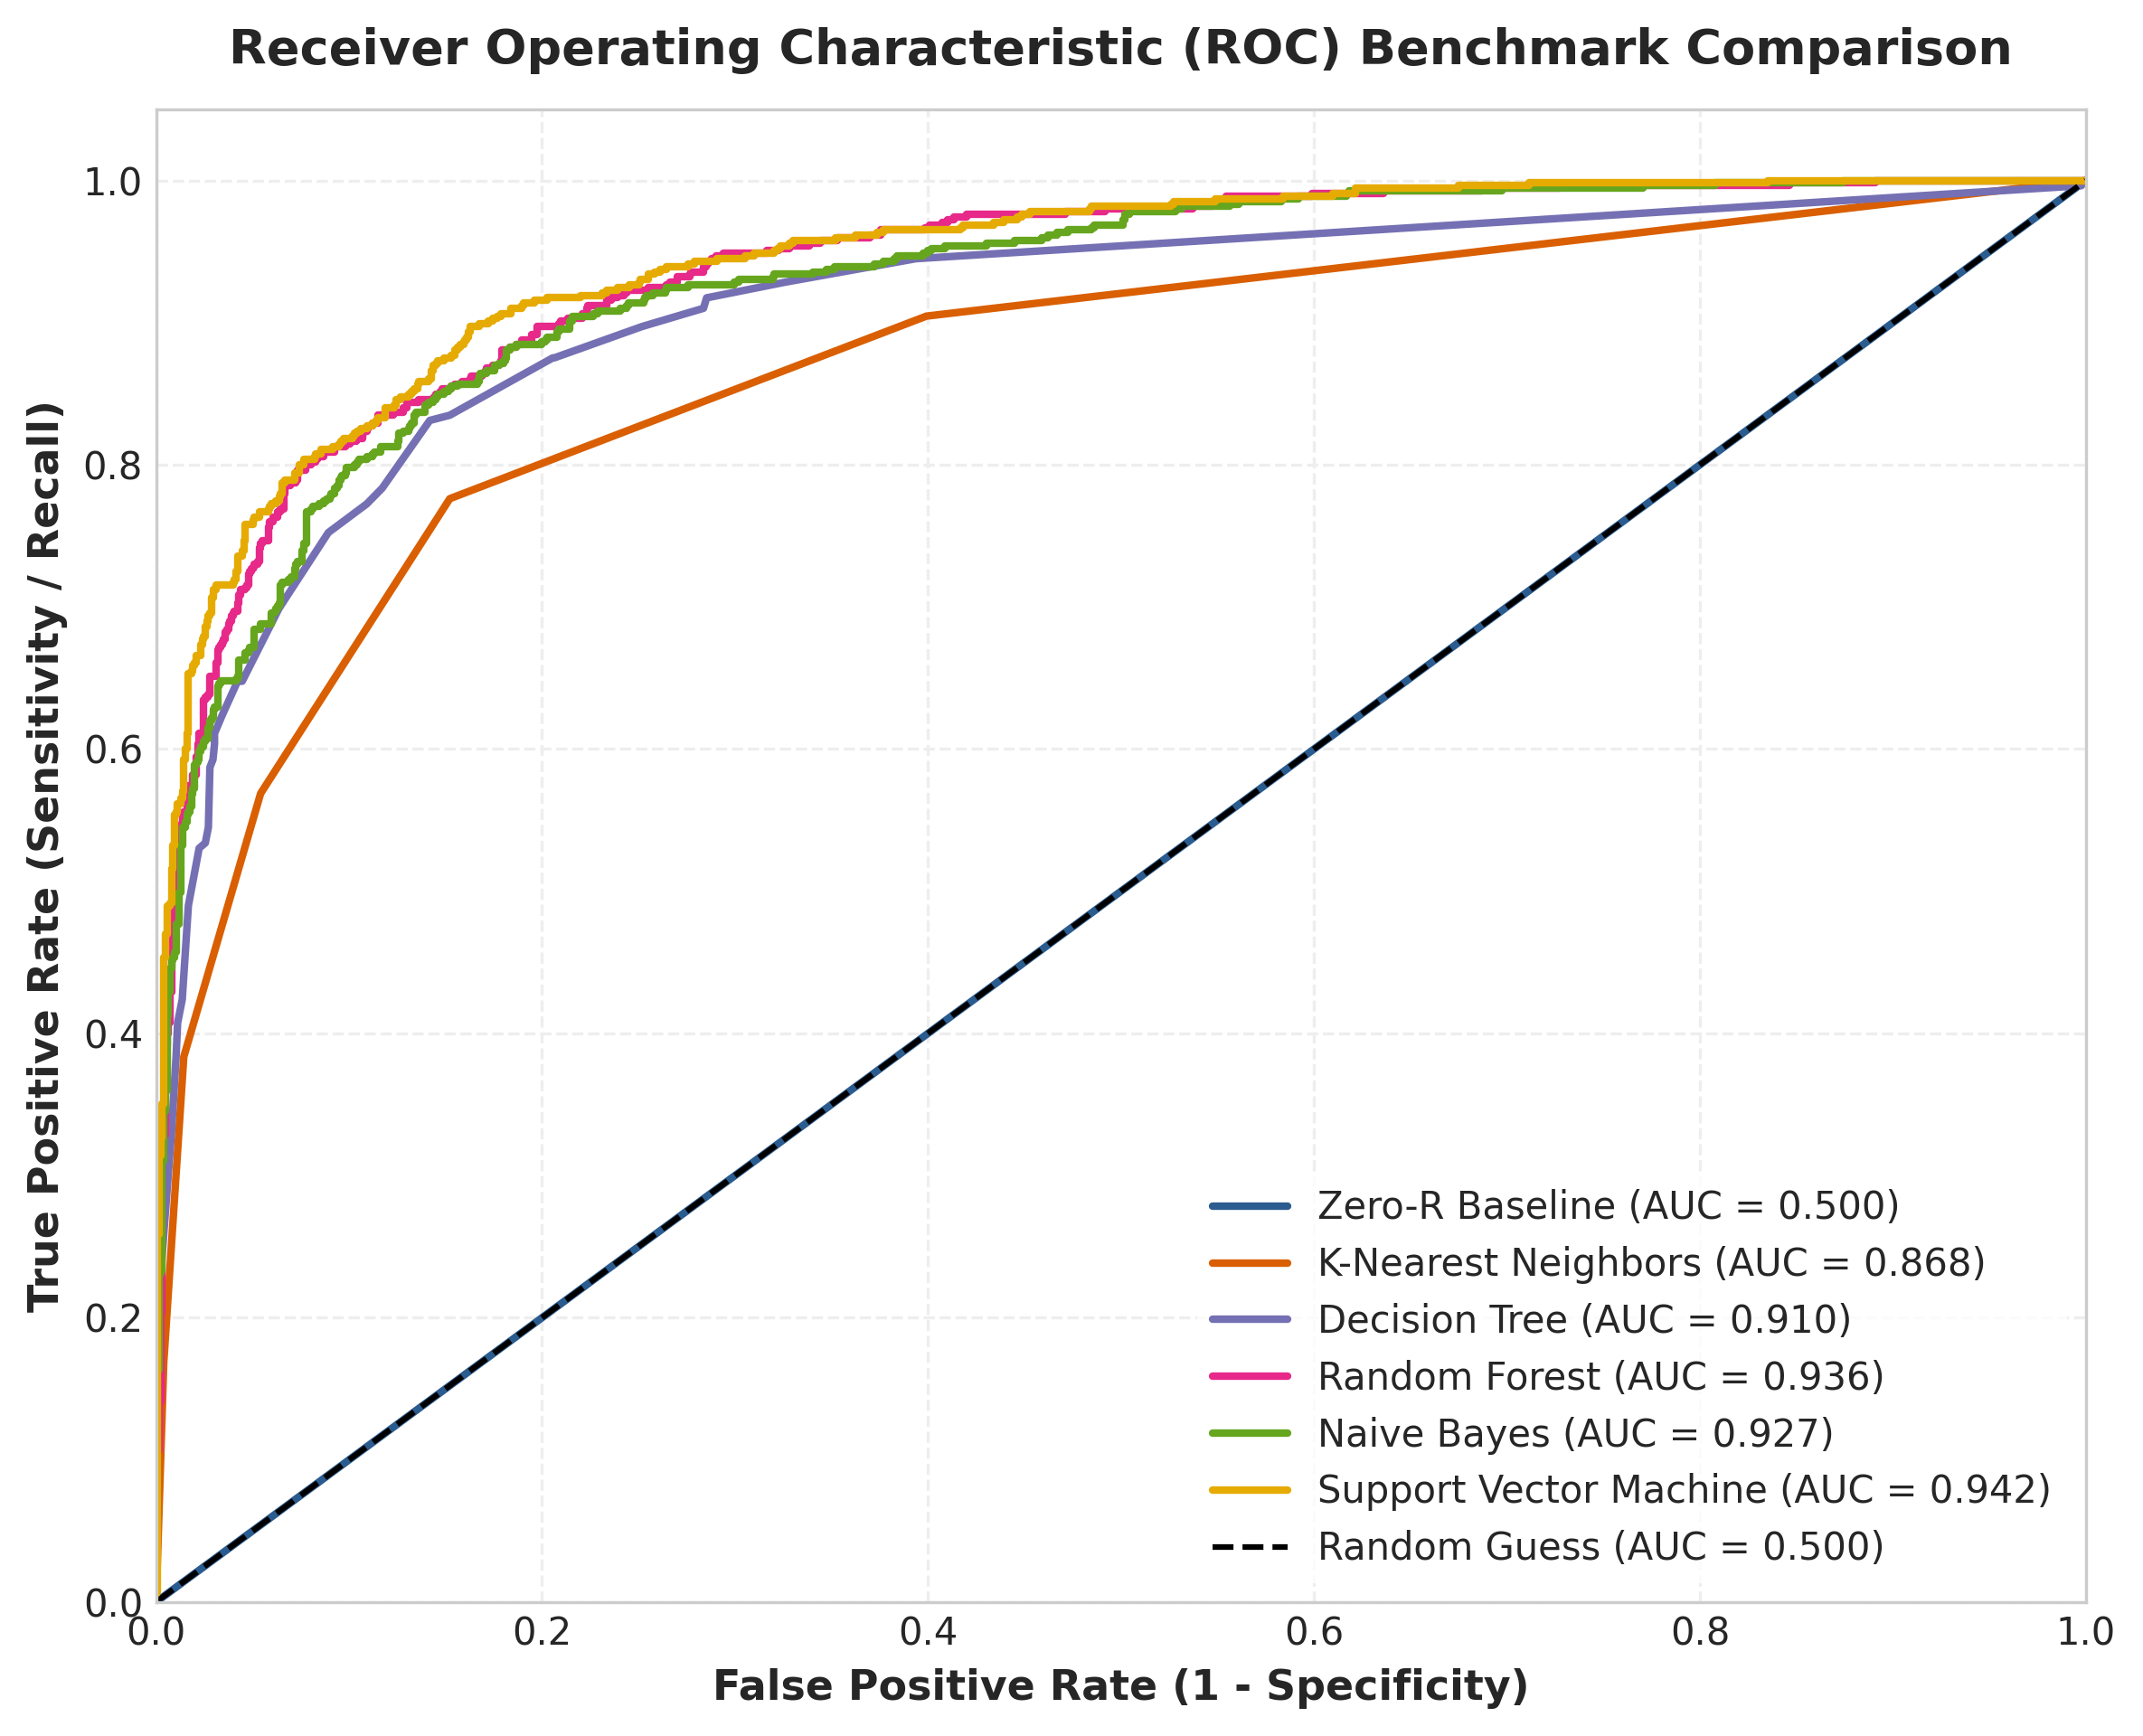
\includegraphics[width=0.75\textwidth]{figures/roc_curves.png}
\caption{Receiver Operating Characteristic (ROC) Benchmark Comparison.}
\label{fig:roc_curves}
\end{figure}

\begin{figure}[H]
\centering
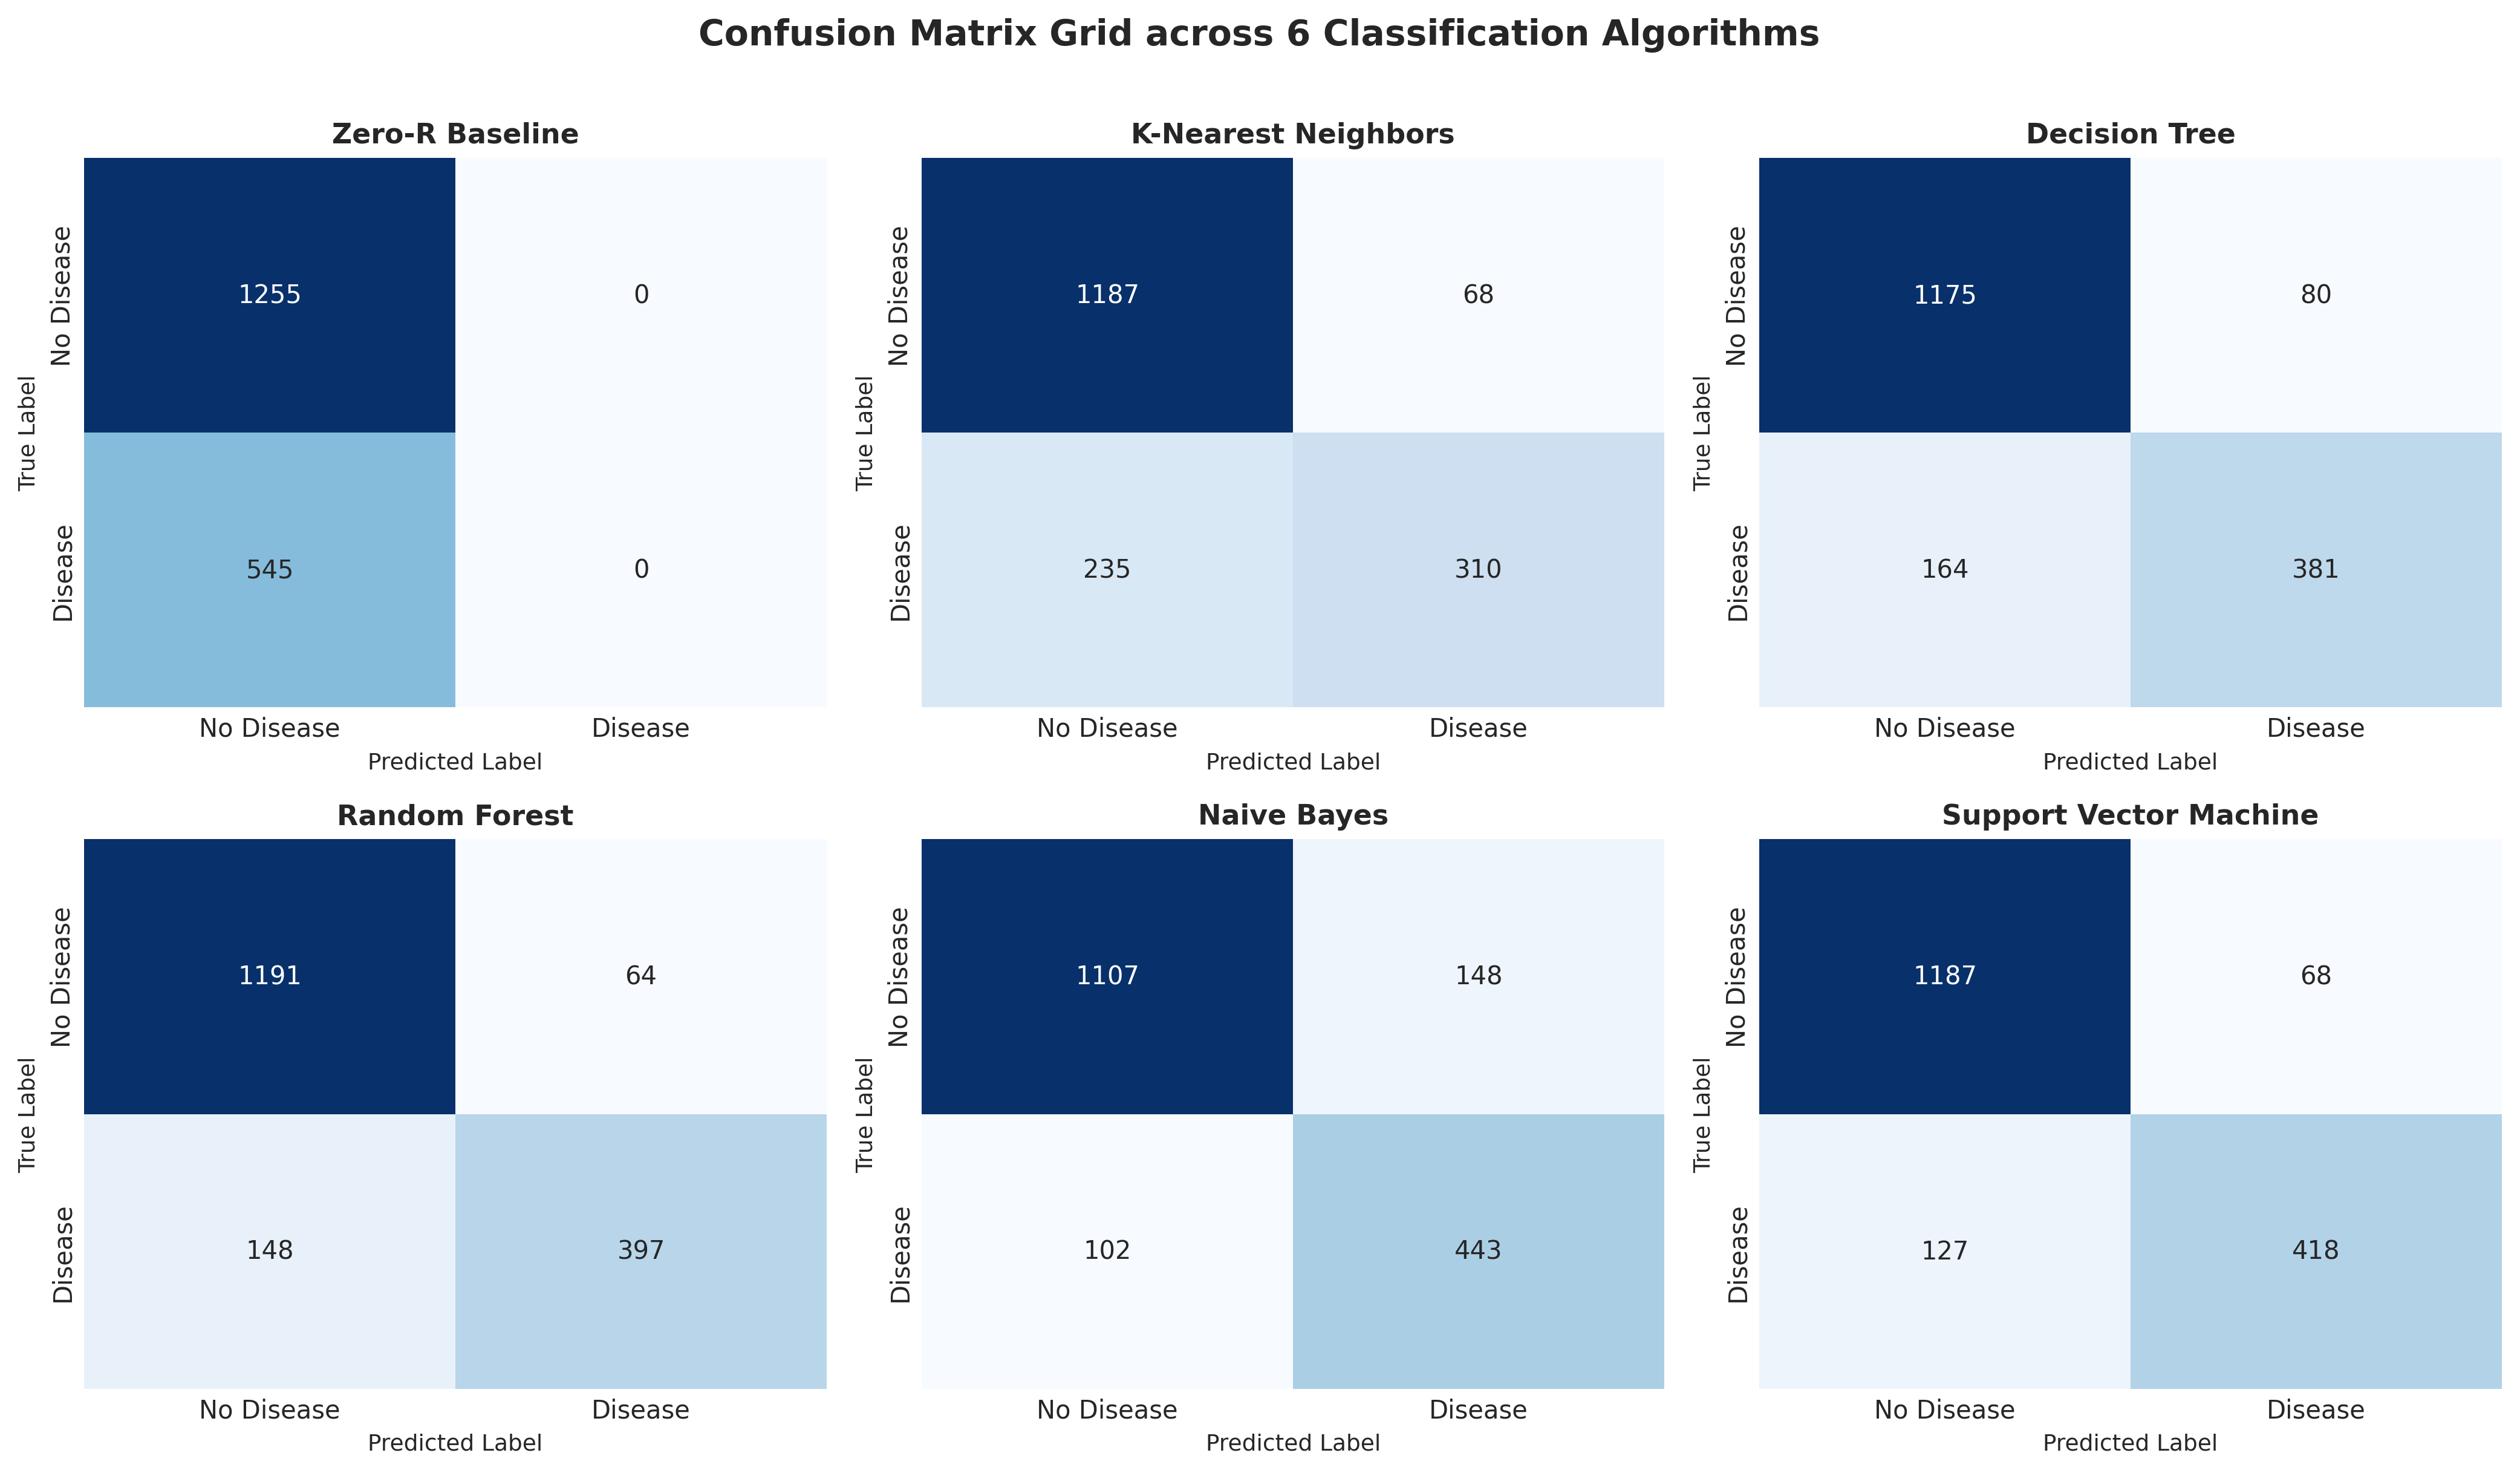
\includegraphics[width=0.8\textwidth]{figures/confusion_matrices.png}
\caption{Confusion Matrix Grid across 6 Classification Algorithms.}
\label{fig:cm_grid}
\end{figure}

\section{Multi-Perspective Feature Importance Consensus}
Figure~\ref{fig:feature_comp} presents a multi-perspective comparison of normalized feature importances across Mutual Information, Random Forest Gini Importance, and Permutation Importance. Maximum Heart Rate Achieved, ST Depression, Age, and LDL Cholesterol consistently form the top predictor cluster.

\begin{figure}[H]
\centering
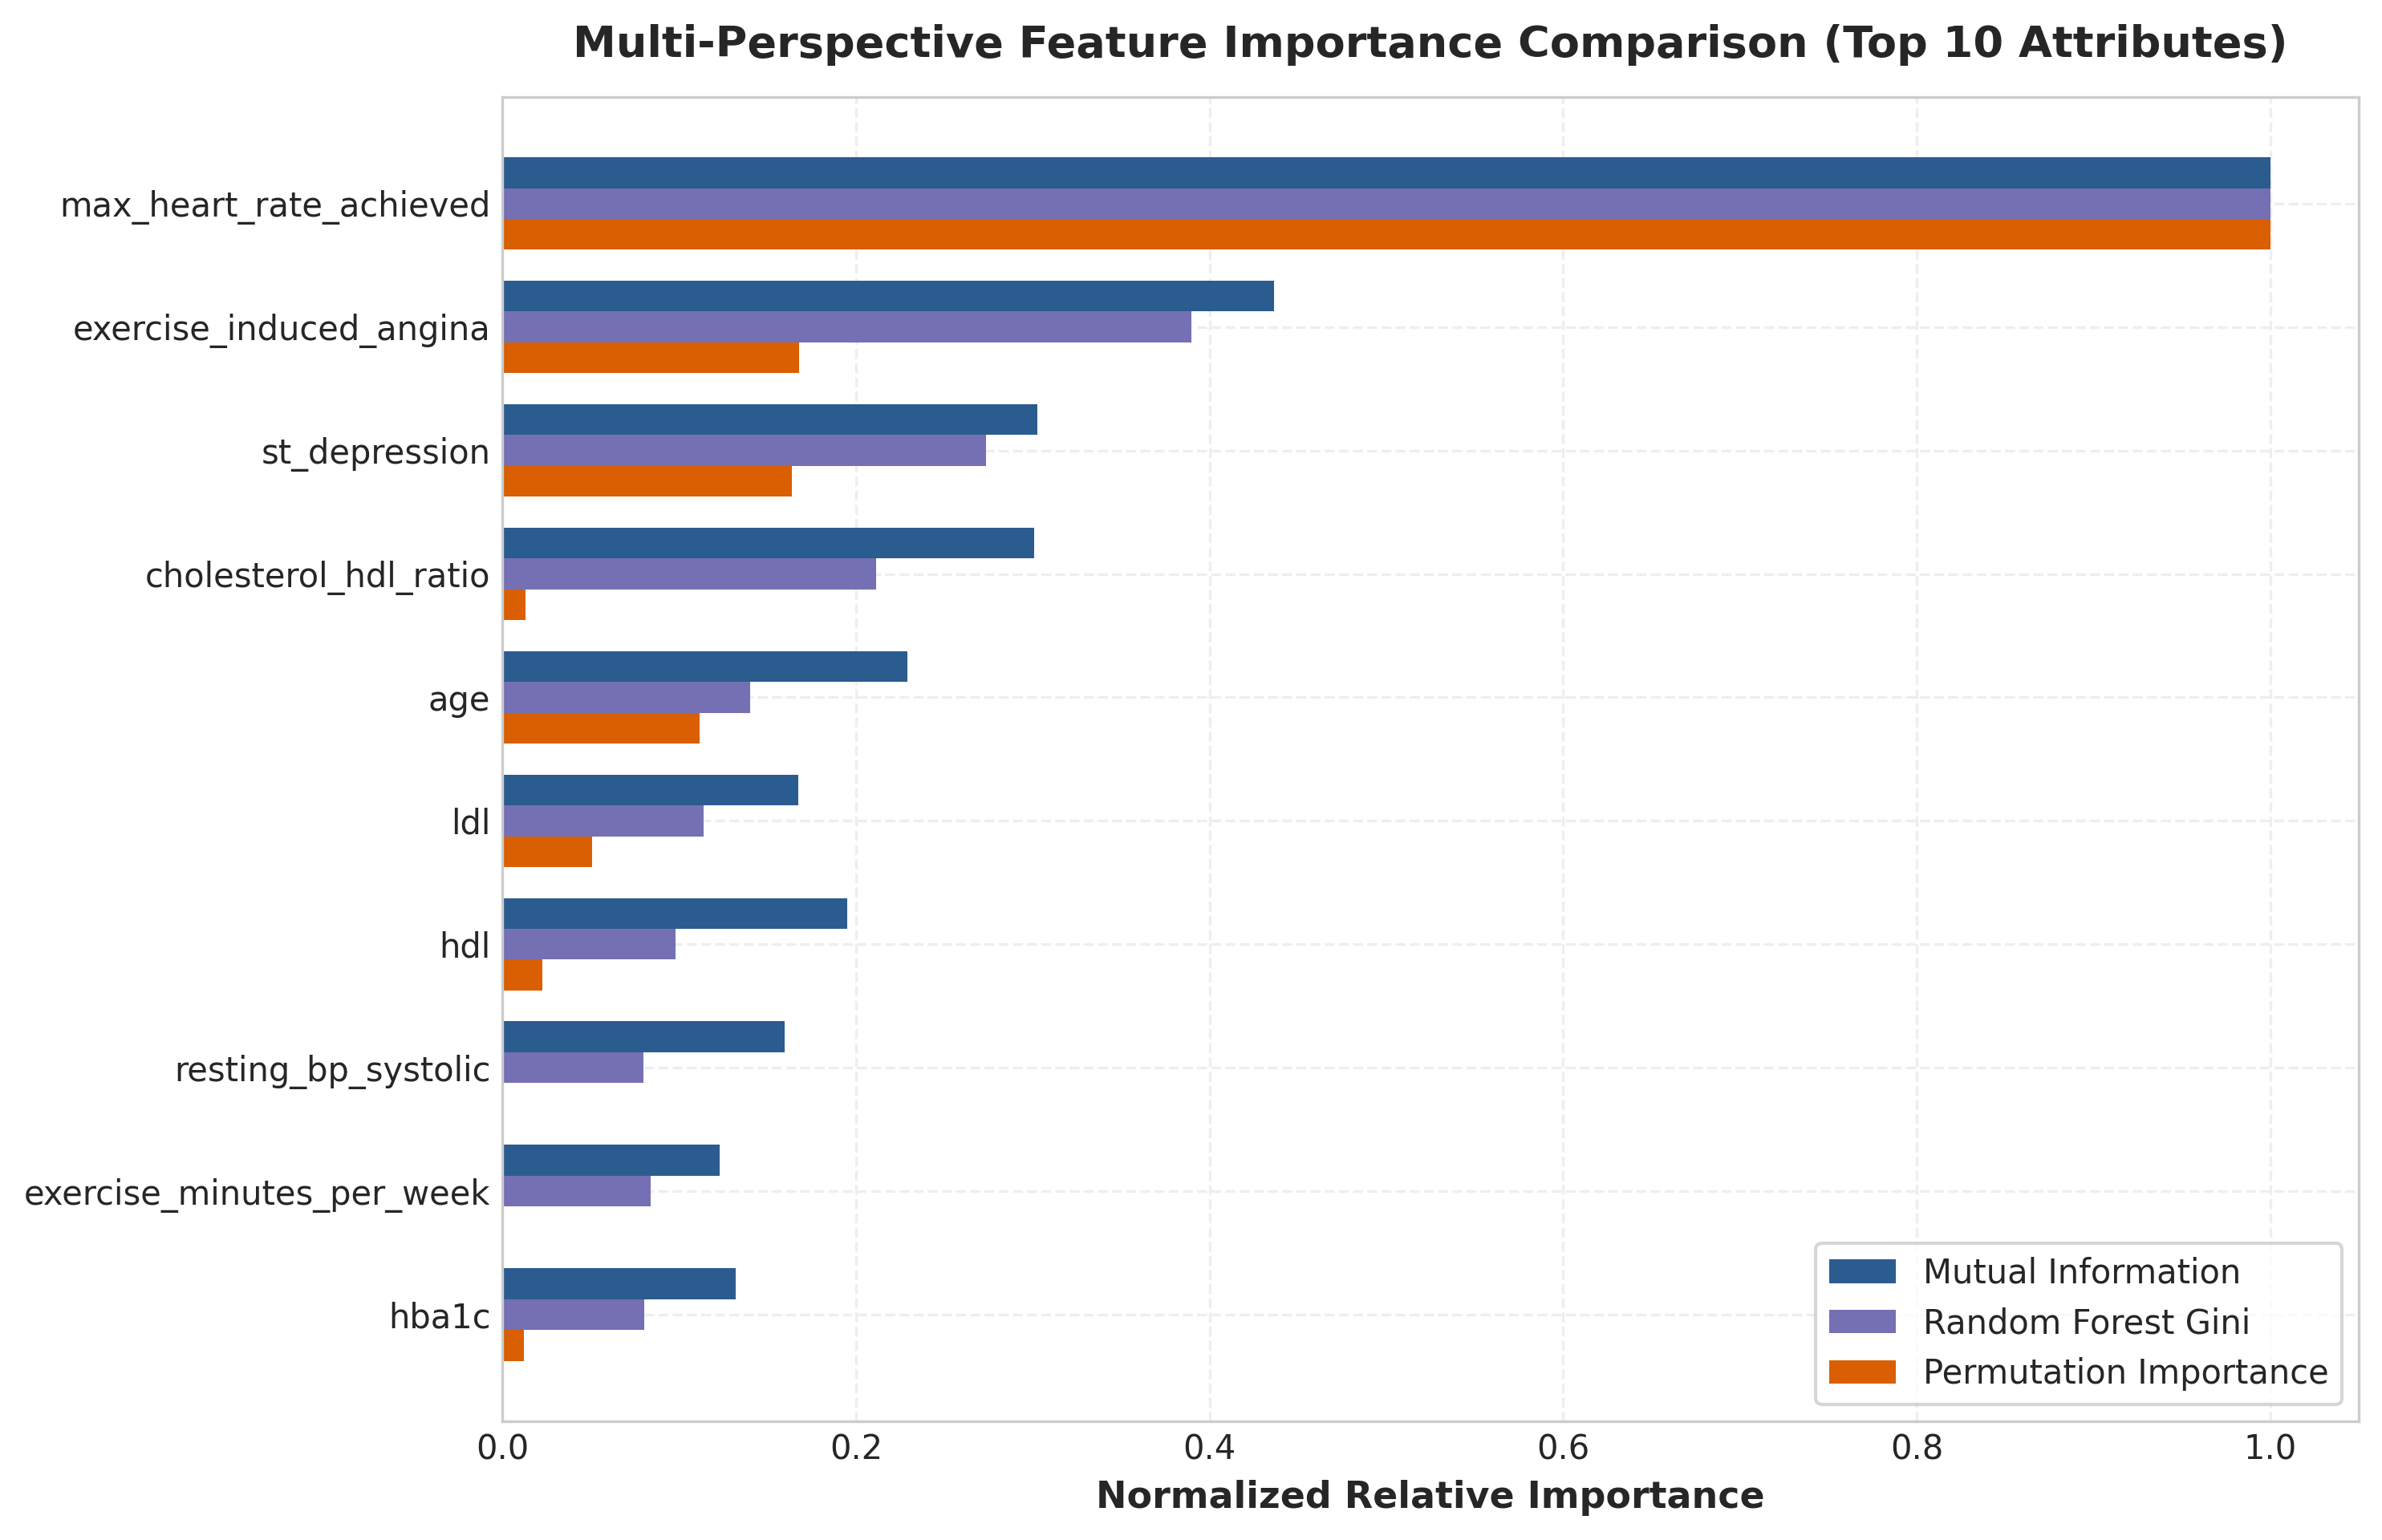
\includegraphics[width=0.8\textwidth]{figures/feature_importance_comp.png}
\caption{Multi-Perspective Feature Importance Comparison.}
\label{fig:feature_comp}
\end{figure}

\section{Healthcare Applications \& Clinical Decision Support}
Machine learning models for cardiovascular risk prediction provide actionable clinical utilities when operationalized into healthcare workflows:

\subsection{Primary Care Triage \& Early Screening}
Routine primary care visits often lack expensive invasive imaging. Machine learning models enable clinicians to input non-invasive parameters (vitals, blood panel, age, chest pain type) during standard consultations to generate immediate risk scores.

\subsection{Personalized Modifiable Risk Interventions}
By identifying top feature importance drivers (LDL cholesterol, smoking status, exercise minutes, diet quality score), clinicians can design tailored behavioral interventions:
\begin{itemize}
    \item \textbf{Lipid Management:} Targeting LDL reduction when blood chemistry features rank high.
    \item \textbf{Exercise Prescription:} Adjusting physical activity plans for patients with chronotropic deficit (blunted peak heart rate).
\end{itemize}

\subsection{Integration with Consumer Wearables}
Modern wearable devices continuously capture daily steps, resting heart rate, sleep duration, and stress scores. Feeding these passive continuous streams into trained predictive models allows remote patient monitoring and automated alert triggers when physiological risk spikes.

\subsection{7-Tier Clinical Risk Stratification Scale}
To translate continuous probabilities $P(Y=1 \mid X) \in [0\%, 100\%]$ into actionable medical triage, we establish a 7-tier clinical risk scale:
\begin{enumerate}
    \item \textbf{$0\% - 15\%$ (All OK / No Risk):} Optimal health profile; routine preventive care.
    \item \textbf{$15\% - 30\%$ (Low Risk):} Low risk profile; standard annual checkups.
    \item \textbf{$30\% - 45\%$ (Medium Risk):} Mild elevation; lifestyle modifications advised.
    \item \textbf{$45\% - 55\%$ (Borderline Risk):} Threshold boundary; secondary diagnostic screening recommended.
    \item \textbf{$55\% - 70\%$ (High Risk):} Substantial elevation; clinical evaluation \& lipid therapy.
    \item \textbf{$70\% - 85\%$ (Very High Risk):} High disease likelihood; cardiologist referral.
    \item \textbf{$85\% - 100\%$ (Critical Danger Zone):} Immediate clinical diagnostic testing (echocardiogram / angiography).
\end{enumerate}

\section{Detailed Empirical Discoveries \& Findings}
\begin{enumerate}
    \item \textbf{Prevalence Profile:} Target disease prevalence is $30.30\%$ ($N=9,000$), demonstrating moderate class imbalance ($2.3:1$) that necessitates Weighted F1 and ROC-AUC metrics over raw accuracy.
    \item \textbf{Chronotropic Response Deficit:} Peak exercise heart rate is severely blunted in heart disease patients ($145\text{ bpm}$ vs $173\text{ bpm}$), exhibiting a large effect size (Cohen's $d = 1.34$, $p < 0.0001$).
    \item \textbf{Myocardial Ischemia Marker:} ST segment depression acts as the top positive clinical marker (Glass Rank-Biserial $r = 0.42$, $p < 0.0001$).
    \item \textbf{Classifier Superiority:} Support Vector Machine (RBF kernel) achieved the highest overall discrimination ($89.17\%$ Accuracy, $0.9422$ ROC-AUC).
    \item \textbf{Synergistic Risk Triad:} Age, LDL Cholesterol, and HbA1c interact non-linearly to compound individual cardiovascular vulnerability.
    \item \textbf{Exercise Angina Odds:} Presence of exercise-induced angina quadruples the odds of positive heart disease diagnosis (Odds Ratio $= 3.425$, $p < 0.0001$).
\end{enumerate}

\section{Limitations \& Medical Disclaimer}
\begin{tcolorbox}[colback=red!10!white,colframe=red!75!black,title=\textbf{MEDICAL DISCLAIMER}]
This paper and associated web application are developed strictly for academic Data Mining demonstration purposes. Its predictions must \textbf{NOT} be interpreted as a medical diagnosis or as a substitute for professional medical advice. Statistical association does not imply clinical causality.
\end{tcolorbox}

\section{Student Contribution Matrix}
\begin{table}[H]
\centering
\caption{Simulated Student Responsibility Matrix}
\begin{tabular}{lll}
\toprule
\textbf{Student Code} & \textbf{Primary Responsibilities} & \textbf{Git Feature Branch} \\
\midrule
AISD05 & Dataset acquisition, quality audit, EDA, hypothesis testing & \texttt{feature/AISD05-eda} \\
SIAD19 & Preprocessing pipeline, ML modeling, tuning, evaluation & \texttt{feature/SIAD19-modeling} \\
RSD20 & Streamlit web application, predictor UI, LaTeX report & \texttt{feature/RSD20-streamlit} \\
\bottomrule
\end{tabular}
\end{table}

\section{Conclusion \& Future Perspectives}
This expanded research study successfully demonstrates an end-to-end Data Mining investigation for heart disease risk classification. Support Vector Machine (RBF kernel) achieved leading diagnostic accuracy ($89.17\%$) and ROC-AUC ($0.9422$). 

\textbf{Future Directions:} Future work includes integrating deep learning tabular architectures (such as TabNet), expanding to longitudinal electronic health records (EHR), incorporating continuous wearable streams, and deploying privacy-preserving federated learning across multi-hospital networks.

\begin{thebibliography}{99}
\bibitem{kaggle2026} Udit Jain, \textit{Heart Disease Risk Dataset 2026}, Kaggle, 2026.
\bibitem{scikit-learn} Pedregosa et al., \textit{Scikit-learn: Machine Learning in Python}, JMLR, 12:2825-2830, 2011.
\bibitem{who2024} World Health Organization, \textit{Cardiovascular Diseases (CVDs) Key Facts}, WHO, 2024.
\end{thebibliography}

\end{document}
